\chapter{Preliminary Work Plan} \label{chap:chap3}

% Academic and industrial setting and data source
\section{Academic and Industrial Setting}

The present work unrolls at Faculdade de Engenharia da Universidade do Porto by a student employee of Enlitia \cite{EL}. One of the employer's requirements is to formulate the final algorithm in the Python programming language \cite{Python}. Therefore, we consider academic and industrial standards during the development of the tool.

Having the possibility of working with a company that provides artificial intelligence solutions for energy systems, there is ample availability of PV asset data from various clients, mainly from the Iberian Peninsula and other European countries. There will be a need to gather information from assets with historical significance and with the presence of faults. Although Enlitia leases PV asset data for this work, its origin will remain classified.

% Work phases
\section{Work timeline}

\begin{figure}[h!]
    \centering
    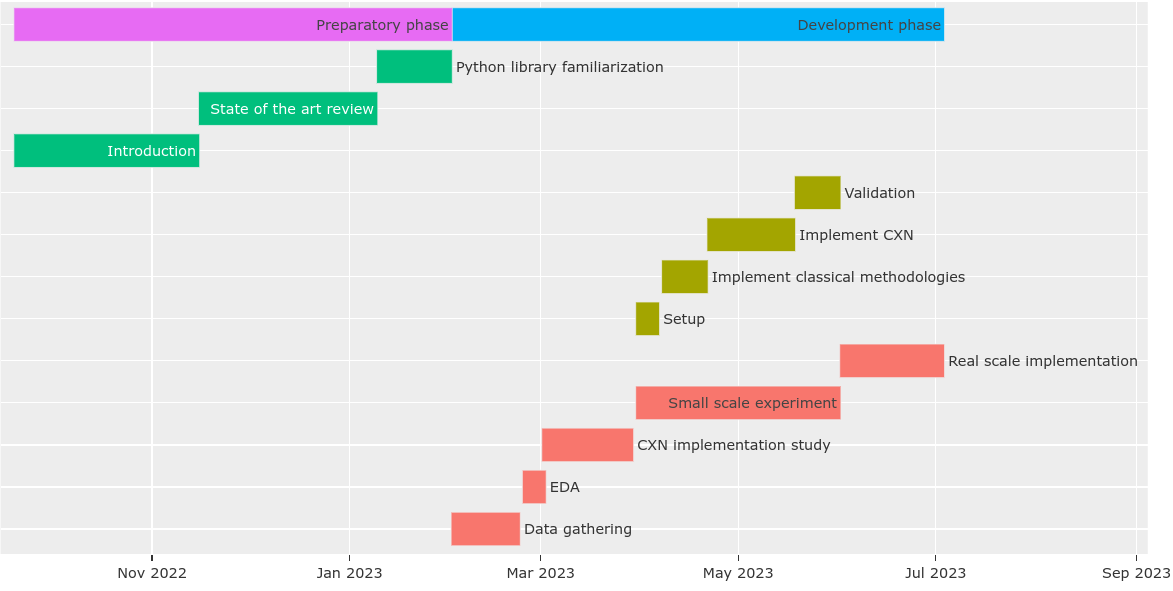
\includegraphics[width=\linewidth]{figures/chapter3/gantt.png} \caption{Dissertation work timeline represented by a Gantt chart.}
    \label{fig:gantt}
\end{figure}

Figure \ref{fig:gantt} represents the expected chronological sequence of events. The most uncertainty comes from adapting the formulation of CXNs for PV fault detection and developing a Python application that implements its behavior, given that the know-how associated with this step is yet to be understood. There is also some doubt about the work time required to upscale the experimental environment toward actual deployment, knowing that the empirical setting of data science experiments may radically differ from software production environments. There will be an attempt to match the development environment with the implementation context, reducing the latter's risk.

% Document structure
According to the predefined workflow, the following chapters of this document will include:

\begin{itemize}
    \item Deep analysis of Cell Complex Neural Networks and adaptation proposals towards PV fault detection and classification algorithms.
    \item The process of data gathering, defining data sources, and available information.
    \item Exploratory data analysis (EDA) and data mining (feature extraction, clustering, etc.).
    \item Setup context for the small-scale experiment: dataset construction, cleaning, normalization pipelines, etc.
    \item Implementation of classical ML methodologies.
    \item Implementation of novel CXN methodology.
    \item Result validation.
    \item Productization of the developed algorithm.
    \item Large scale deployment of the application.
\end{itemize}

% Strategies
\section{Development strategies}

Data gathering will be accomplished by combining as many data sources for the same variables as possible, such as power meters and SCADA measurements, local meteorological stations, and satellite data. Then, datasets will be organized into specific categories according to time resolution, acquisition method, availability, and accuracy. Geographical-based characterization might also be utilized to divide data even further. Data analysis, feature extraction, and clustering are essential in this step to harness valuable data from unlabeled samples.

To implement classical ML methodologies, as well as the proposed tool, Python libraries such as TensorFlow \cite{tensorflow}, Scikit-learn \cite{sklearn}, and SciPy \cite{scipy} are the finest selection. They facilitate the creation of neural networks and other learning structures, possessing many different implementations of scientific algorithms. Other utilities discovered during the development process will be referenced along.

Software engineering guidelines will rule the software architecture of the final application, which should follow its well-studied organization patterns. Even though it is not a focus of this work, paying attention to code implementation should result in a better application, scalability, and security.

% Final product

\section{Final expectations}

The final application aims to implement online fault detection for operational PV assets. For performance reasons, its deployment architecture is a consideration to take in prior, such as its potential for parallelization. It should be as generalized as possible, as that would increase its correct functioning for different PV assets of various plant operators. In the end, it is expected to resemble the usability and robustness of a finished software product so that PV plant operators can reliably utilize its outputs. Its success will result in higher PV system efficiencies and safety, advancing the world's energy transition.

% \chapter{Conclusions}

% Given the current state of investment in grid-connected big-scale photovoltaic systems, it's known that resource allocation to fault recovery is essential to meet grid code requirements, safety, and health standards, reduce investment risk and maximize the asset's throughput. The literature supported this claim by presenting extensive research on fault detection and classification in PV systems. These works have utilized various methodologies ranging from image-based to electrical-based approaches and incorporated techniques such as signal processing, graph theory, statistics, machine learning, deep learning, and even quantum machine learning. Different authors have used the same dataset and small-scale research facility, providing some data consistency across multiple studies. However, many have also relied on synthetic validation data with unrealistic operating scenarios. To combat this issue, and since this work encompasses PV systems with differing characteristics from most (utility-scale instead of small-scale or simulated), the development phase will cover a comparative analysis of some of the most relevant methodologies utilizing a common (and realistic) dataset. Finally, it aims to develop a novel approach to fault detection and classification in PV systems using contemporary deep learning techniques (CXN). The results of this research will contribute to a better understanding of fault occurrence and accurate fault classification in PV systems, supporting their growth as a reliable and efficient renewable energy source.